Randomized algorithms are algorithms that use a degree of randomness as part of their logic. Randomized algorithms frequently outperform and simplify the best-known deterministic algorithms, and sources of randomness are a powerful but evasive resource. Further, access to randomness is an essential tool for cryptography. Randomized algorithms are designed and studied under the assumption that computers have access to true randomness in the form of a sequence of truly random bits. However, this randomness is taken from sources that only appear to have randomness, otherwise known as entropy. Entropy is a term borrowed from physics that refers to the amount of "disorder" in a system and is the measure of the uncertainty associated with a random variable. Some examples of these sources of randomness are generating and measuring electromagnetic or radioactive noise, measuring the timing of past events, or measuring user-dependent behavior \cite{Shaltiel2011}. The goal of randomness extraction is to convert these weak sources of randomness into uniformly random bits, which are measured in terms of the min-entropy. A visual representation of this process can be seen in \autoref{fig:HighlevelDiagram}. This has led to the research and development of Classical Randomness Extractors (CC-Extractors). In Section 2, we give a thorough introduce the two main concepts of Classical Randomness Extractors, deterministic and seeded extractors. %%% [Final Report] We000 briefly discuss about few construction of CC extractor. 

\begin{figure}[!htb]
    \centering
    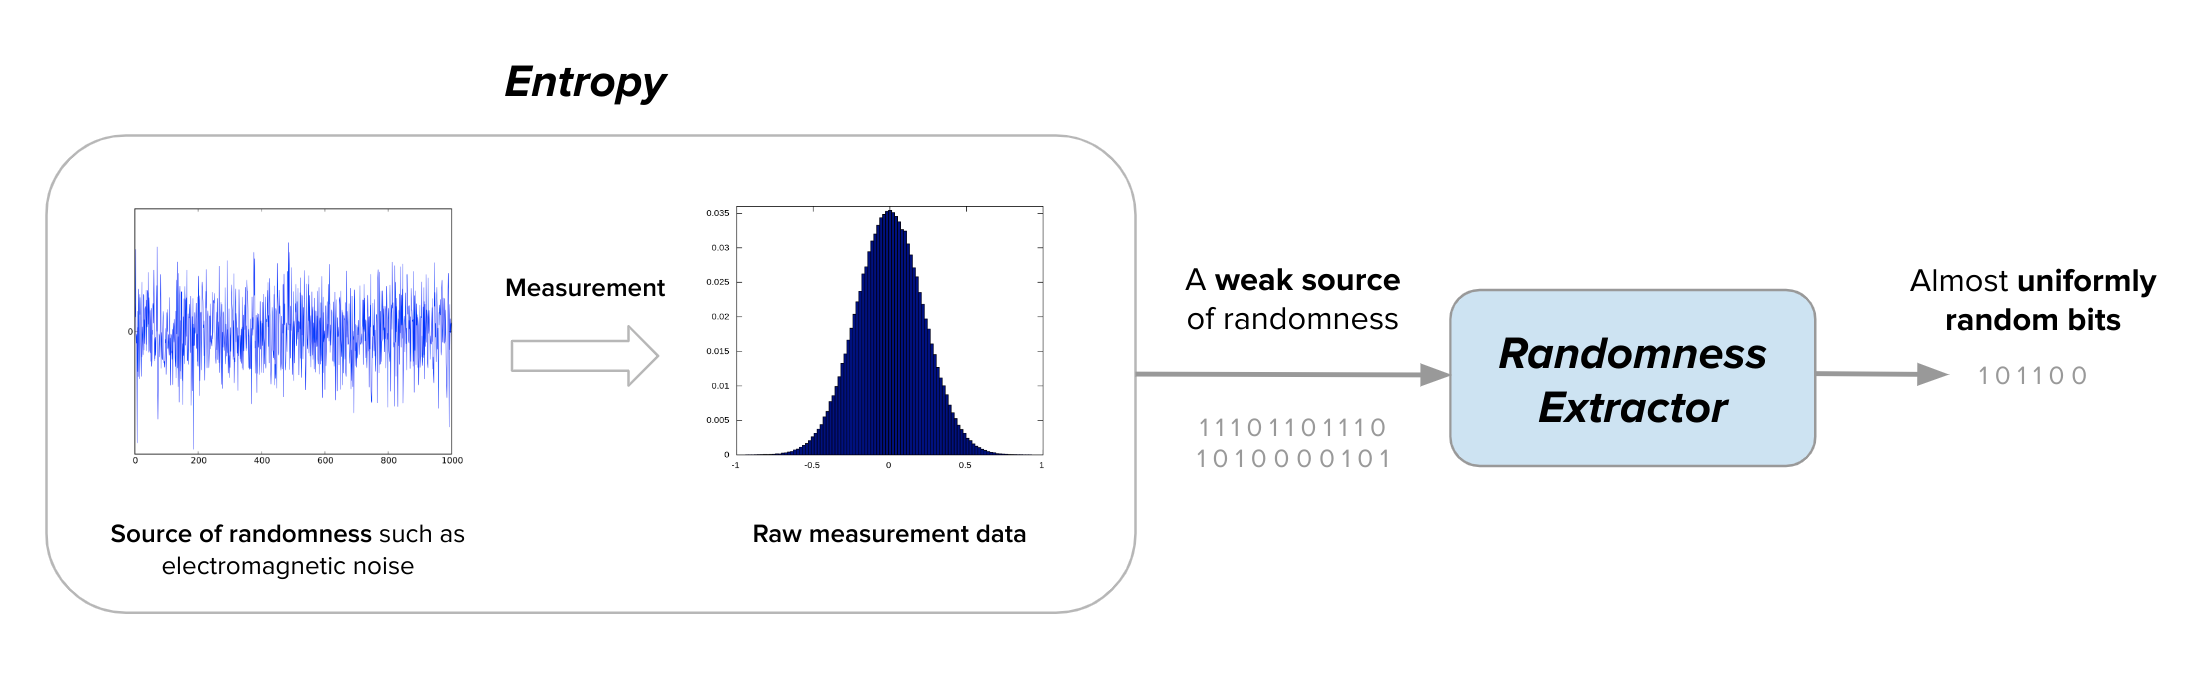
\includegraphics[scale=0.18]{Images/Highlevel_extractor.png}
    \caption{High-level diagram of a randomness extractor}
    \label{fig:HighlevelDiagram}
\end{figure}

We now know, however, that the underlying world is not classical but rather quantum, resulting in the development of quantum mechanics. %% add references
Subsequently, a randomness extractor may hold quantum side information about its (almost) uniformly random output sequence, $X$. This realization lends to several questions: where do $X$ come from? How can we hope to harness even weak sources to obtain a surplus of classical randomness? How much randomness can we obtain from a quantum source rather than a classical string? \cite{Berta_2014} Questions such as these have culminated in the study of Quantum-to-Classical Randomness Extractors (QC-Extractors) with the goal of determining how we can extract classical randomness from a physical source by performing measurements on the quantum state of said source. In contrast to the classical world, quantum mechanics allow for the creation of true randomness given the correct circumstances. It is also important to note that in a quantum setting, there also exist Quantum-to-Quantum Randomness Extractors (QQ-Extractors) that we do not measure but determine if the resulting state is quantumly fully random (maximally mixed) and uncorrelated from the extractor. In Section 3, we introduce the necessary background quantum preliminaries, and in Section 4, we discuss the construction and evaluation of QC and QQ Randomness Extractors.

Finally, we will conclude our report in Section 5 by examining the applications of QC-Extractors to entropic uncertainty relations and cryptographic problems such as noisy storage models, and Section 6 where we explore future directions of this work. Entropic uncertainty relations are fundamental to quantum mechanics and crucial tools for quantum cryptography. We will provide and discuss the proof from \cite{Berta_2014} that any set of measurements forming a QC-extractor yields an entropic uncertainty relation with respect to quantum side information and thereby obtain relations both for the Shannon and the min-entropy. The second application we will discuss is proving security in the noisy-storage model. The noisy-storage model is a quantum cryptographic model that assumes an adversary is imperfect or noisy. The study of QC extractors can further be extended to other cryptographic problems, for example, privacy amplification. We refer the curious reader to the following articles, lecture notes, and textbooks \cite{Berta_2014,tudelftQC,lo2007quantum,bruss2007quantum, bernstein2009introduction,bennett1992quantum,berta2013quantum,wilde2013quantum,nielsen2002quantum} for further reading on quantum cryptography.    